\chapter{Adaptación de la implementación}

\label{chap:adaptacion}

\section{Implementación Base}

Para poder empezar a adaptar la AWD-LSTM a los requerimientos necesarios, se decidió arrancar con una implementación del modelo de lenguaje obtenida de \textit{GitHub}\footnote{https://github.com/ahmetumutdurmus/awd-lstm}. Esta implementación se eligió frente a otras debido a que esta se encontraba actualizada a las nuevas versiones de la librería \textit{pytorch}, permitiendo así una mejor capacidad de adaptación a las mejoras futuras. En particular el repositorio presentaba una estructura bastante simple, compuesto por 4 archivos principales que daban forma a la arquitectura completa de la AWD-LSTM:

\begin{itemize}
    \item \textit{main.py}: Archivo el cual contenía la lógica del entrenamiento del modelo, permitiendo tunear los hiperparámetros del mismo. Previamente al entrenamiento, en este mismo también se extraían los \textit{datasets} de entrenamiento, testing y validación a partir de importarlos localmente. Luego, estos se dividían en \textit{batches} para poder entrenar al modelo final y validarlo durante las distintas épocas. Para finalizar, el estado del modelo se guardaba cada vez que se lograba encontrar un modelo mejor al finalizar una época. En el caso de que se quisiera interrumpir el script durante el entrenamiento, el código que englobaba al mismo presentaba manejo de excepciones frente a una interrupción voluntaria del usuario, deteniendo el entrenamiento y devolviendo la \textit{perplexity} del último modelo guardado frente al \textit{dataset} de testing.
    \item \textit{finetune.py}: Archivo casi idéntico al anterior, utilizado para reentrenar el modelo en el caso que se preste necesario. Sus principales diferencias recaían en que este archivo permitía inicializar el modelo con alguno ya entrenado previamente, cargando los pesos de la red neuronal a partir de un diccionario que almacenaba el estado de la misma. Además otra característica de este proceso de reentrenamiento es que no estaba implementado de manera que se le pueda indicar al mismo que este reentrene al modelo por una cantidad fija de épocas, sino que él mismo las haría indefinidamente hasta que la condición no monotónica del optimizador se cumpla.
    \item \textit{ntasgd.py}: Archivo el cual definía el optimizador del modelo.
    \item \textit{model.py}: Archivo el cual albergaba todas las clases que en su conjunto representaban a la red neuronal completa que define a la AWD-LSTM. En este mismo se definen todas las capas de la arquitectura, además de especificar cómo se propaga para adelante la entrada de la red, alimentando así los pesos de la misma durante el entrenamiento.
\end{itemize}

Esta implementación presentaba una serie de hiperparámetros los cuales se podían variar para generar distintos modelos de lenguaje. Para más información sobre los mismos o sus valores predeterminados, consultar el anexo \ref{sec:hiperparametros}. A menos que se indique lo contrario, durante la realización de este trabajo estos serán los valores por defecto que se utilizaran para cada uno de los experimentos.

Por otro lado, yendo más en detalle sobre el archivo \textit{main.py}, en particular sobre de qué manera el programa prepara el corpus de texto para poder alimentar al modelo durante el entrenamiento, se pudo observar que este funciona de una manera un poco particular (Figura \ref{fig:armado_texto}).

\begin{figure}[htb]
    \centering
    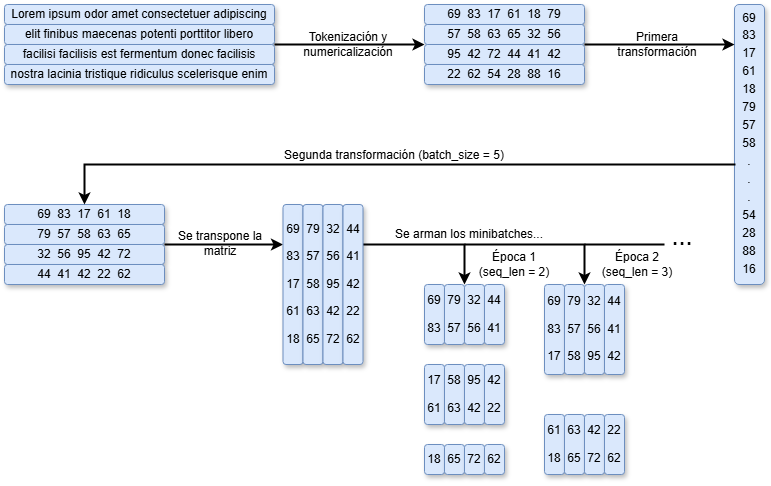
\includegraphics[width=1\textwidth]{imagenes/armado_texto.png}
    \caption{Pipeline usado para generar el \textit{batch} que alimentará al modelo durante el entrenamiento.}
    \label{fig:armado_texto}
\end{figure}

En primer lugar, se separa al corpus de texto en oraciones, donde cada oración se divide en una lista de \textit{tokens}: palabras (sin signos de puntuación, en minúscula, y sin dígitos ni caracteres no romanos) y signos de puntuación, más la introducción de ciertos caracteres extra para brindar más información sobre el contexto de la palabra, desde caracteres que permiten indicar que la palabra siguiente empieza con mayúsculas hasta caracteres que indican el fin de una oración (tokenización). Cada uno de estos \textit{tokens} está representado por un único número (numericalización). Estas listas de números (es decir, las oraciones) son transformadas en un tensor de una única columna con tantas filas como \textit{tokens} haya presentes en la Figura \ref{fig:armado_texto}. Este tensor luego es nuevamente transformado, esta vez en un tensor con una cantidad de filas igual a la cantidad de \textit{batches}. Previamente, con el objetivo de que la cantidad de palabras sea divisible por esta cantidad de lotes y el redimensionamiento del tensor sea posible, se descartaba un pedazo del corpus del final del texto. Una vez hecho esto, se transpone el tensor, quedando una cantidad de columnas igual al tamaño del \textit{batch}.

Por último, para alimentar al modelo, se separan estos \textit{batches} en lotes aún más pequeños, llamados \textit{minibatches}, dependiendo del tamaño de la secuencia que se use en esa época, ya que este tamaño es variable y se recalcula cada vez que se inicia una de ellas \parencite{merity2017regularizingoptimizinglstmlanguage}.

\section{Validación de Implementación Base}

\label{sec:validacion_base}

Una vez presentada la implementación base, se buscó estar seguros de que la misma se comportaba de manera similar en cuanto a capacidad de predicción con una implementación de AWD-LSTM. Para poder averiguar empíricamente esta cuestión, se decidió comparar la implementación base obtenida con la implementación proveída por la librería de \textit{Python} denominada \textit{Fastai}, la cual presenta diversas arquitecturas de modelos de lenguajes. Sin embargo, como esta no permite la modificación de su estructura a nivel red neuronal, se la había descartado como implementación base.
Previamente a esto, se modificó la forma en la cual la LSTM tokeniza y numericaliza los textos, usando también la librería \textit{Fastai} para tokenizarlos, no solo por comodidad, sino también debido a que esta genera nuevos \textit{tokens} de acuerdo a distintos contextos. A futuro esta modificación también serviría en términos de tiempo de ejecución y espacio de memoria, ya que la implementación base obtenía los \textit{tokens} seleccionando el texto completo y transformándolo en un conjunto de palabras, lo cual para corpus muy grandes no sería factible. Los resultados de la comparación se pueden encontrar en la experimentación correspondiente.

Con nuestra implementación empíricamente validada, se continuó la adaptación modificando la forma en la que el modelo recibe el corpus de entrenamiento. En un principio este recibía el corpus a partir de un archivo local. Con el objetivo de poder entrenar la LSTM con textos sustancialmente más grandes en tamaño, lo que se hizo fue adaptar la implementación con una clase llamada \textit{Corpora}, utilizada en trabajos previos en el laboratorio para generar conjuntos de corpus de texto, permitiendo agregar los mismos de manera local o de manera remota a partir de un repositorio de \textit{Huggingface}. De esta manera, sería posible no solo entrenar el modelo con un corpus remoto, como es el caso de \textit{Wikipedia}, sino también reentrenar el modelo con los \textit{scanpaths} generados por los experimentos de movimientos oculares.

Otro cambio que se aplicó a la implementación relacionado a los corpus, fue la eliminación del corpus de testing, para simplificar el código, ya que no lo veíamos pertinente para las experimentaciones futuras. Con esto dicho, en resumidas cuentas para el entrenamiento del modelo la implementación quedó con dos corpus, uno de entrenamiento y otro de validación, correspondientes al 80\% y 20\% del \textit{dataset} original respectivamente. Esta división se hizo de manera aleatoria utilizando una semilla para permitir la replicabilidad de los experimentos en un futuro.

\section{Métricas}
Para poder probar el comportamiento de nuestro modelo a futuro con las experimentaciones, en este trabajo nos hemos centrado en dos métricas generales:

\begin{itemize}
    \item \textit{Perplexity}: La cual se utilizó para medir la capacidad predictiva entre distintos modelos de LSTM, basados en un mismo vocabulario.
    \item \textit{Correlación con juicios de valor humanos}: Utilizando la correlación de \textit{Spearman} y la distancia coseno para averiguar si los \textit{embeddings} generados por la LSTM son capaces de captar las mismas similitudes entre pares de palabras que los capturados por los seres humanos. En caso de querer ver más en detalle cómo se genera esta correlación, ver sección \ref{sec:experimentos_similitud}.
\end{itemize}

Para la primera métrica, la implementación base ya presenta con la capacidad de poder calcular la \textit{perplexity} del modelo a lo largo del entrenamiento. Sin embargo, para obtener la segunda métrica se necesita una manera de obtener \textit{embeddings} a partir de la LSTM. A priori, el modelo no es un modelo dedicado a devolver los \textit{embeddings} de un vocabulario en particular como Word2Vec, sino más bien es un modelo dedicado a predecir la siguiente palabra dado un contexto. Afortunadamente, la arquitectura AWD-LSTM presenta una capa de \textit{embeddings} dentro de la red neuronal, por lo cual el siguiente cambio que se realizó a la arquitectura es el de, una vez finalizado el entrenamiento del modelo, extraer esta capa de \textit{embeddings}, la cual es una matriz de tamaño vocabulario por dimensión del \textit{embedding}, el cual es un hiperparámetro del modelo. 

Una vez extraídos los \textit{embeddings} de la red, estos eran copiados en un archivo de texto en un formato que permita utilizar los \textit{embeddings} para ser importados por librerías como \textit{Gensim}. Así, será sencillo hacer la comparación con otros \textit{embeddings}. El formato (Figura \ref{fig:archivo_embedding}) consiste en:

\begin{itemize}
    \item Como primera línea del archivo se encuentran las dimensiones de la capa de \textit{embeddings}.
    \item En las siguientes líneas aparecen, una por cada palabra del vocabulario, la palabra en sí junto a su \textit{embedding}, separadas por un espacio en blanco.
\end{itemize}

\begin{figure}[htb]
    \centering
    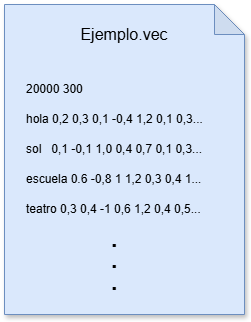
\includegraphics[width=0.35\textwidth]{imagenes/archivo.png}
    \caption{Ejemplo de archivo de texto donde se guardarán los \textit{embeddings} resultante del entrenamiento. En este caso, 20000 sería el tamaño del vocabulario mientras que 300 es el tamaño del \textit{embedding}.}
    \label{fig:archivo_embedding}
\end{figure}

Además, para poder tener una idea más detallada de cómo evolucionan estos \textit{embeddings} a medida que se entrena la LSTM, se tomó la decisión de no solo extraer los \textit{embeddings} finalizado el entrenamiento, sino al terminar cada época del mismo. Luego, estos serían comparados con los juicios de similitud de \textit{Multi-Simlex}, obteniendo la correlación entre los mismos en cada época.

\section{Incorporación de movimientos oculares al modelo}

Como mencionamos previamente, el objetivo principal de este trabajo es el de observar la performance del modelo, luego de añadirle información sobre los movimientos oculares de personas durante la lectura del texto con el cual se está alimentando al mismo. Para poder cumplir esto entonces, se decidió hacer una modificación a la red neuronal clásica de la arquitectura AWD-LSTM. Basados en la idea del aprendizaje multitarea, se tomó la decisión de obligar al modelo a que no solo prediga la siguiente palabra dado un contexto, sino que también prediga las métricas relacionadas con movimientos oculares que más se han estudiado en la literatura: \textit{First Fixation Duration} (FFD) y \textit{First Pass Regression Time} (FPRT, también llamado \textit{Gaze Duration}) (ver \ref{subsec:metricas_movimientos} para su definición).

Yendo más en detalle, se añadió una capa extra en el modelo, compuesta por una regresión lineal, la cual recibe el \textit{batch} con el cual se está alimentando en ese momento a la red y devuelve un resultado. Una vez hecha la predicción, con el objetivo de que la misma vaya mejorando a lo largo de las épocas, se la compara con las métricas reales obtenidas del experimento utilizando el error absoluto medio como función de pérdida. En los casos en donde no existieron métricas relacionadas a movimientos oculares se tomó la decisión de directamente no comparar esta predicción generada, para así no influir en el entrenamiento del resto de la red.

\section{Problemas de memoria}

\subsection{Primera transformación}

Luego de haberse realizado testeos preliminares para asegurar el funcionamiento de la LSTM de manera correcta, el proyecto se topó con un problema importante a solucionar. El código original de la implementación, especialmente en la sección en donde se acondiciona el corpus para transformarlo en un \textit{dataset} adecuado, para luego ser separado en \textit{batches} de texto que serían enviados a la LSTM durante el correr de las épocas, no estaba preparado para poder manejar corpus de gran tamaño. 

Como se mencionó anteriormente, durante la ejecución los corpus eran transformados en un tensor de 1 sola columna y 1 fila por cada palabra que compusiera el mismo, para luego ser nuevamente transformados de acuerdo al tamaño del \textit{batch}. Luego de examinar el código detenidamente, se llegó a la conclusión que existía un problema en esta primera transformación, ya que se hacía utilizando las herramientas básicas del lenguaje de programación y no apoyándose en las librerías externas que dieran un mejor uso de la memoria, haciendo que a medida que se iba generando el tensor, la memoria de la computadora se fuera llenando, llegando a terminar el programa abruptamente cuando el tamaño del corpus era lo suficientemente grande.

Como esto no permitía que la LSTM pudiera ser entrenada con textos extensos, se buscó una manera de mejorar el uso de la memoria en este paso del programa. La solución propuesta fue la de aprovecharse de la interfaz de la librería \textit{Huggingface}, la cual no solo permite la importación de corpus de entrenamiento, sino que también provee una simple interfaz para poder realizar transformaciones sobre el \textit{dataset}, permitiendo así poder replicar la primer transformación del corpus, a la vez de reducir en gran medida el consumo de la memoria en este paso en particular, ya que la herramienta permite ejecutar la transformación de manera paralela dentro de la memoria. Incluso se aprovechó esta herramienta para poder realizar la tokenización y numericalización del corpus, reduciendo no sólo espacio sino tiempo, al también proveer la posibilidad de ejecutar las transformaciones de manera paralela entre varios hilos de ejecución.

Estas modificaciones permitieron que la LSTM se pudiera entrenar con porcentajes cercanos al 30\% de un corpus de texto que contenía alrededor de 28 millones de oraciones. Sin embargo, como los experimentos realizados con otros modelos como Word2Vec se habían llevado a cabo con la totalidad de ese corpus, se decidió probar de entrenar el modelo con un porcentaje mucho mayor.

\subsection{Segunda transformación}

Desafortunadamente, se pudieron observar de vuelta problemas de memoria al entrenar con la totalidad del corpus. Al analizar más en detalle el porqué de esto, nos dimos cuenta que el programa se detenía previo a la segunda transformación mencionada anteriormente, o sea, la que dividía al \textit{dataset} en \textit{batches}. También se encontró un pico de uso de la memoria cuando se accedía al \textit{dataset} en particular, dando la pauta de que el acceso al \textit{dataset} tampoco se estaba haciendo de manera eficiente en este caso.

Un primer enfoque el cual se tomó fue el de recurrir a la librería \textit{PyTorch} y utilizar los \textit{dataloaders} que esta provee, permitiendo un acceso del \textit{dataset} de a \textit{batches} y evitando tener que colocarlo entero en memoria. Esta idea traía un problema crucial: el \textit{dataloader} va generando lotes cuyo texto es contiguo en el corpus, lo cual es evitado en el código original utilizando las transformaciones anteriormente mencionadas, ergo, el conjunto final de \textit{minibatches} resultaba distinto.

Como se buscó mejorar el uso de la memoria del modelo sin alterar íntegramente la lógica del código, se decidió ir por otra solución. Esta solución implicó la utilización de nuevo de la librería \textit{Huggingface} y otro de sus elementos que provee para la alimentación de modelos de lenguaje con corpus de datos extensos, el uso del \textit{sharding} \bb{(Figura \ref{fig:sharding}).}

\begin{figure}[htb]
    \centering
    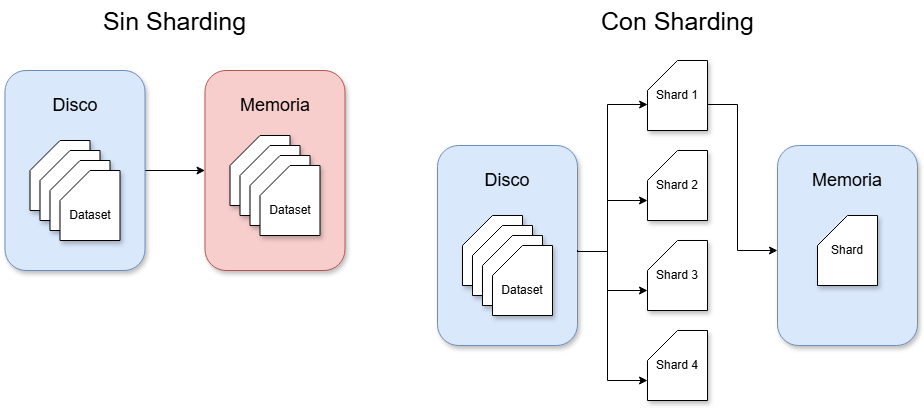
\includegraphics[width=1\textwidth]{imagenes/sharding.png}
    \caption{Sharding, consiste en dividir el \textit{dataset} en fragmentos más pequeños, permitiendo un uso más eficiente de la memoria, ya que lo que ingresa en la memoria es el fragmento y no el \textit{dataset} entero.}
    \label{fig:sharding}
\end{figure}

En particular, en este caso previo a la realización de las transformaciones para generar los \textit{minibatches}, el \textit{dataset} era dividido en una cantidad fija de fragmentos (modificable como parámetro del \textit{script} de entrenamiento), para luego realizar el entrenamiento del modelo de manera normal con el primero de ellos, hasta llegar al último, donde terminado este se daría como finalizada la época. Esto generó mejoras sustanciales en el uso de la memoria, permitiendo el entrenamiento de la LSTM con el 100\% del \textit{dataset} con el uso de 5 fragmentos. No solo eso, sino también permite a futuro poder aumentar la cantidad de fragmentos en el caso de que este modelo se quiera entrenar con un corpus aún más grande.

\subsection{Red neuronal}

Para finalizar, también se hizo una modificación a cómo computa la red neuronal los resultados. En particular, previo a la capa en donde se encuentran las celdas LSTM, se encuentra la capa de \textit{embeddings}, donde el \textit{batch} de palabras que se envían como entrada es transformado en sus respectivos \textit{embeddings}, luego de aplicarse un \textit{dropout} de algunos de estos \textit{embeddings} con el objetivo de reducir el sobreajuste. En esta capa, sin embargo, se descubrió que la manera en que se hacía esto en la implementación original era ciertamente ineficiente en términos de memoria.

\begin{figure}[htb]
    \centering
    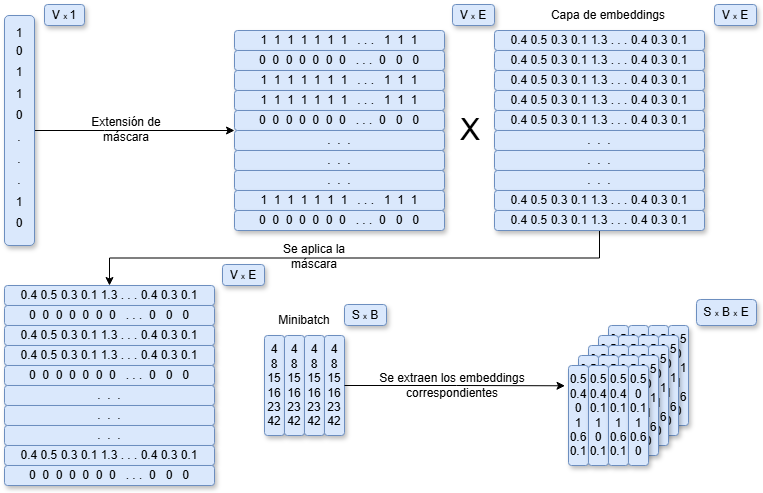
\includegraphics[width=1\textwidth]{imagenes/algoritmo_viejo.png}
    \caption{Algoritmo original para extraer los \textit{embeddings} de la capa de \textit{embeddings}, donde $V$ es el tamaño del vocabulario, $E$ es el tamaño del \textit{embedding}, $B$ es el tamaño del \textit{batch} y $S$ es el largo de la secuencia}
    \label{fig:algoritmo_viejo}
\end{figure}

Para empezar, en la implementación se genera una máscara de una dimensión, del tamaño del vocabulario ($V$), en la cual cada punto corresponde a una palabra en particular y es marcada con un 1 o un 0 de acuerdo a una distribución de bernoulli. Luego esta máscara es extendida a una matriz de dimensión $V + E$ (donde $E$ es el tamaño de los \textit{embeddings}), literalmente copiando los valores anteriores en memoria cuantas veces sean necesarios. No solo eso, además esta máscara es multiplicada celda por celda con la capa de \textit{embeddings} de la red neuronal, deshabilitando algunos \textit{embeddings} de manera aleatoria, pero generando a su vez otra matriz provisoria de tamaño $V + E$. Por último se extraen los \textit{embeddings} de esta matriz provisoria para cada uno de los \textit{tokens} del \textit{batch}. Esta implementación nos pareció ineficiente, especialmente en casos en donde $V$ es grande, pudiendo llegar a ocupar gran parte de la memoria de la GPU innecesariamente (Figura \ref{fig:algoritmo_viejo}).

\begin{figure}[H]
    \centering
    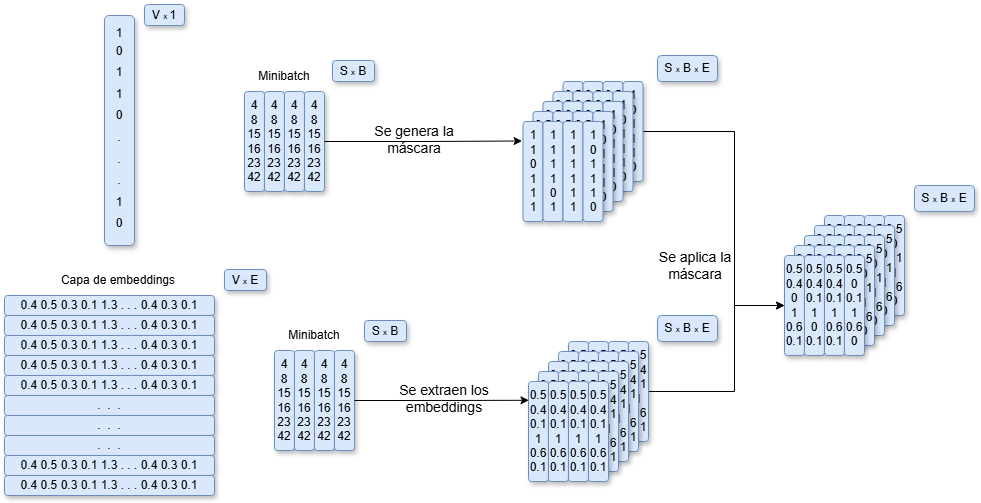
\includegraphics[width=1\textwidth]{imagenes/algoritmo_nuevo.png}
    \caption{Optimización del algoritmo para extraer los \textit{embeddings}. Se definen las mismas variables que en el caso anterior.}
    \label{fig:algoritmo_nuevo}
\end{figure}

Para solucionarlo, se decidió ir por otra implementación más optimizada. En este caso, no se extendió la máscara y se mantuvo como un tensor de una sola dimensión. Luego, directamente se extraen para el \textit{batch} en cuestión los \textit{embeddings} de la capa, generando un tensor de 3 dimensiones, esta vez de tamaño $S \times B \times E$ (donde $S$ es el largo de la secuencia y $B$ el tamaño del \textit{batch}). Además, se genera otro tensor, esta vez solamente de tamaño $S \times B$, donde dentro de él se encuentran los resultados de la máscara para \textit{token} del \textit{batch}, indicando si esa palabra debería ser deshabilitada o no. Por último, se multiplican celda por celda ambos tensores, en definitiva multiplicando ya sea por 1 o por 0 cada uno de los \textit{embeddings} del mismo. Si analizamos detenidamente las dimensiones resultantes de los dos algoritmos, podemos ver, teniendo en cuenta que $S \times B << V$, que los tensores intermedios del segundo algoritmo son mucho más pequeños que los del algoritmo original, ergo ocupando menos espacio de la memoria de la GPU.

\section{Abstracción del código}

Pudiendo ya entrenar sin problemas el modelo con el corpus, se decidió realizar varios cambios estructurales a los archivos con el objetivo de simplificar el código, mejorar la lectura del mismo y poder incorporarlo al sistema original del proyecto, el cual permitía el entrenamiento de otras arquitecturas de manera general, como Word2Vec.

El primero de los cambios fue el de abstraer el código del archivo \textit{main.py} dentro de una clase \textit{AwdLSTM}. Luego, al notar que el código perteneciente al archivo \textit{finetune.py} era idéntico al de su contraparte, se decidió abstraer aún más la clase, transformándola en la interfaz de una jerarquía de clases. Esta jerarquía estaría conformada por una clase \textit{AwdLSTMForFinetuning} y otra llamada \textit{AwdLSTMForTraining}, encargadas del reentrenamiento y entrenamiento del modelo respectivamente. Dentro de estas clases sólo se encuentran las funcionalidades específicas a esa etapa del modelo. Las funcionalidades que se compartan entre estas dos serían englobadas por la interfaz \textit{AwdLSTM}, evitando así código repetido.

Además, aprovechándose de la similitud entre las dos clases, se incorporó polimorfismo a la jerarquía, permitiendo que se simplifique el código aún más al utilizar en funcionalidades que comparten las dos, métodos cuya implementación dependerá del estado del modelo en el que esté. El código se encuentra publicado en \textit{Github}\footnote{https://github.com/FerminT/LMET} para su consulta.

\section{Modificaciones dentro del reentrenamiento}

Una vez ya adaptada toda la etapa de entrenamiento, nuestro siguiente objetivo fue el de modificar la etapa de reentrenamiento para poder arrancar con la experimentación. Un primer cambio fue el de modificar la LSTM para que esta implemente un método estático que funcione como \textit{factory method}, pudiendo así englobar la funcionalidad de generar la clase que define al modelo en un contexto de entrenamiento o en un contexto de finetuning en un solo lugar.
Otra cosa que se hizo fue modificar el criterio de corte del modelo cuando este está finetuneando. En un principio, el reentrenamiento no se hacía durante una cantidad fija de épocas, sino que este terminaba cuando la LSTM alcanzaba la condición no monotónica del optimizador, lo cual con la idea en mente de simplificar el código, se decidió modificar y dejarlo igual a como actúa la LSTM en un contexto de entrenamiento.
Por último, se aseguró que el vocabulario presente en los textos de reentrenamiento estuviera presente en el vocabulario del modelo final. Para eso, en la etapa de entrenamiento se añadió como parte del vocabulario no solo las palabras presentes al corpus de entrenamiento, sino también todas las palabras presentes en el corpus utilizado durante los experimentos de movimientos oculares.



